\documentclass[table,a4paper,oneside]{book}

\usepackage{graphicx} % Allows insert of graphics
\usepackage{longtable} % Allows for multipage spanning tables
\usepackage{pdfpages} % Simplifies insertion of multipage PDF'’s
\usepackage{natbib} % Puts in bibliography style
\usepackage[pdfborder=0 0 0]{hyperref} % Adds PDF links
\usepackage{mathptm} % Changes font
\usepackage{fancyhdr} % Allows the use of the fancy Header package
\usepackage{url} % Makes URL's appear nicer and follow formatting rules
\usepackage{algorithm} % Allows Algorithmic insertions to be floated
\usepackage{algorithmic} % Allows Algorithms and Pseudocode
\usepackage{textcomp} % LaTeX support for the Text Companion fonts.
\usepackage{setspace} % Allows the use of the set space command
\usepackage{listings} % Allows the use of source code
\usepackage{colortbl} % Adds colour to rows etc
\usepackage{acronym} % Allows the use of acronyms in code - deals with printing acronyms out nicely
\usepackage[a4paper,vmargin={25.4mm,25.4mm},hmargin={35.0mm,25.4mm}]{geometry} % Allows the changing of page borders

\setlength{\parindent}{0.0in} % Sets paragraph indentation to 0
\pagestyle{fancy}
\bibpunct{(}{)}{,}{a}{,}{,} % Defining the citation style
\newcommand{\degree}{\ensuremath{^\circ}} % Sets new command - Inserts degree symbol
\newcommand{\HRule}{\rule{\linewidth}{0.5mm}} % Set new command - Add blank line
\newcommand{\mtwo}{m\textsuperscript{2} } % Sets the command - Adds m^2.

% Acronym Definition
% \acrodef{label}[acronym]{written out form}
% \acrodef{acronym}{written our form}
\acrodef{ADB}{Approved Document B}
\acrodef{BCIS}{Building Cost Information Service}
\acrodef{CLG}{Department of Communities and Local Government}
\acrodef{CSV}{Comma Separated Value}
\acrodef{DSS}{Decision Support System}
\acrodef{FPA}{Fire Protection Association}
\acrodef{FRS}{Fire and Rescue Service}
\acrodef{GUI}{Graphical User Interface}
\acrodef{IRS}{Incident Reporting System}
\acrodef{IRMP}{Integrated Risk Management Plan}
\acrodef{RIBA}{Royal Institute of British Architects}

\begin{document}
\onehalfspacing
% Above command sets document to 1.5 line spacing
% Remove all above when creating thesis from Master document

\chapter{Literature Review}
\label{chapter:Lit_Review}
\acresetall

\section{Introduction}
\label{sec:Introduction}
This chapter details the previous work done in and around the area of Fire Engineering by other academics and research staff. This section identifies the research gap that this research is intended to fill.
\\
\\
Fire engineering covers a broad aspect of research, from investigation into costs, materials, construction methods and the psychology of occupants during fires. This chapter covers the research done in these areas, though mainly in regards to construction and costs of fires. It also includes a brief literature review on the construction of a software tool as this was the predicted outcome of this research.

\section{Fire Protection}
\label{sec:Fire_Protection}
Society dictates that people should be able to enjoy a reasonable level of safety during day to day activites and as such, part of this is protection from natural and man made phenomena such as fire. Such demands for safety, espcially after large incidents where a considerable loss of life or property occurred, led to the initial development of the fire building regulations \citep{Stollard1994}. These building regulations developed over time into the current form we have today in the UK \citep{Communities2006}. These regulations are in place so that the building can be designed safely to allow occupants to escape should a fire occur and to prevent excessively quick fire spread, again, allowing for escape. This focus on life safety is the main concern behind the current regulations and appears to have been reasonably successful, as fire deaths have declined steadily over the past decade \citep{DepartmentforCommunitiesandLocalGovernment2010}. However, there has been a steady increase in the cost of fires over the same period \citep{AssociationofBritishInsurers2009}. These figures seem to show that whilst the building regulations seem to be working for reducing and keeping the number of fire deaths low, their doesn't seem to be any reduction to the cost of fires by constructing to meet the building regulations.
\\
\\
Whilst Approved Document B lays down the building regulations in relation to fire safety and details the easiest method of meeting these regulations, it is by no means the only method of meeting the regulations. Designers also have aceess to two British Standards that set out methods of meeting the regulations. These British Standards are more advanced methods of designing buildings and therefore are used in the larger and more complex buildings. These two codes are also more open in how the design of the building can attain fire safety certification. BS 9999: Code of Practice for Fire Safety in the Design Management and Use of Buildings \citep{BSI2008} is a relatively new code that attempts to make it easier for designers to incorporate fire safety into more complex structures without having to use PD 7974: Application of Fire Safety Engineering Principles to the Design of Buildings \citep{BSI2003a} which is used in the most complex of buildings because it reduces fire safety to the first principles of fire science and requires an understanding of flame spread, fire dynamics and combustion science to use effectively.
\\
\\
To meet the fire regulations, buildings have to be protected by differenting fire protection systems. These systems delay the spread of fire and make it easier for the occupants to escape. The design of the building itself and the restriction in the use of combustible materials is one method of preventing fire spread is the main aspect behind the regulations. This method of preventing fire spread is refered to as passive fire protection, as the protection does not need to change state to complete it's function in preventing fire spread. However, additional systems are installed, such as fire alarms and extinction systems are installed and these are active fire protection measures. The combination of both active and passive measures provides the complete fire protection design for a building. Previous research has suggested that the includsion of active measures such as sprinklers can reduce the passive protection measures included in a building \citep{Baldwin1974} though it's still believed that both systems should be used complimentarly \citep{Haack2004}.
\\
\\
There has been much work on the use of active protection measures in buildings, espcially sprinklers \citep{Hall2010,Melinek1993299,Vaidogas2011,Melinek1993} and investigating the costs of sprinklers in various buildings, such as in car parks \citep{Li2004}, residential properties \citep{Butry2009}

\section{Decision Support Systems}
\label{sec:DSS}
A \ac{DSS} can be defined as a ``computer based systems that help decision makers confront ill-structured problems through direct interaction with data and analysis models'' \citep{SpragueWatson198906}. These systems allow designers and managers to access help in the decision making process.
\\
\\
The majority of \ac{DSS} tool have similar features in common. These are:-
\begin{itemize}
\item They are non routine and involve frequent \emph{ad hoc} analysis, fast access to data and generation of non standard reports
\item They often address ``What if?'' questions
\item They have no obvious correct answer; a manager has to make qualitative trade offs and take into account situational factors
\end{itemize}

These features are discussed in Value Analysis: Justifying Decision Support Systems \citep{Keen1981}. This paper disucsses the fact that \ac{DSS} tools are helpful in the role they play but are difficult to quantify in regards to cost savings. However, Keen describes that tools should be:-

\begin{enumerate}
\item Flexible
\item Easy to use
\item Responsive
\item Communicative
\end{enumerate}

He explains that it should be flexible to handle different situations, easy to use so it can be put into different users workflow, responsive as it must not impose a structure on the user and be rapid in its calculations and communicative so that the end user can get the knowledge they need from the tool qucikly and easily. By following these four ``rules'', the tool should be of the most use to the end users.
\\
\\
In his book \citep{Keen1980} , Keen describes the percieved benefits of a \ac{DSS} system. These are:

\begin{enumerate}
\item Increase in the number of alternatives examined
\item Better understanding of the business
\item Fast response to unexpected situations
\item Ability to carry out \emph{ad hoc} analysis
\item New insights and learning
\item Improved communication
\item Control
\item Cost savings
\item Better decisions
\item More effective teamwork
\item Time savings
\item Making better use of data resources
\end{enumerate}

Not all of these 12 benefits can be applied to the design tool in this research, however the proposed tool does achieve a number of these points, specifically points one (alternative approaches), eight (cost savings), nine (better decisions), eleven (time savings) and twelve (Making better use of data resources). By allowing the end user to run more alternatives to the fire design, it is hoped that a better, more cost effective solution can be put forward as an alternative to the other plans a designer might submit.

\section{Data Collection}
\label{sec:Data_Collection}
Most of the data for this PhD is incident data and has already been collected by the \ac{FRS} for \ac{CLG} use as well as the data from the \ac{FPA}. However, data needs to be collected from fire engineers and those involved within the building industry to investigate the current practise and how the fire protection is specified in a building, as based on literature, the mindset appears to be that the structurcal engineer designs the structure and the architect and fire engineer design the fire protection \citep{Alfawakhiri2005}. Collecting data will allow the \ac{DSS} to focus on those that are responsible for the design of the fire protection within a building and therefore the tool can be customised to the needs of that intended group.

\section{Software Design}
\label{sec:Software_Design}
As the outcome of the research is a proposed methodology for a \ac{DSS} system, then a brief literature review should cover the design of the software. The tool is designed to be used by fire engineers and possibly fire engineering clients, so the tool will cater to the needs of the fire engineers. The definetion of tool in this research follows that given by Lockley and Sun \citep{Lockley1995} which is ``a computer program that is used by engineers to perform analysis of a building or its services (prior to relisation) for the purpose of making, modifying or evaluating design decisions''.

\subsection{User Interface}
\label{sec:User_Interface}

As discussed in \ref{sec:DSS}, Keen puts forward the areas a \ac{DSS} should follow to allow the best use. These were that it should be flexible, easy to use, responsive and communicative. These aspects are met in the coding of the software. For example, ease of use comes down to the design of the \ac{GUI}. A well developed \ac{GUI} will allow users to navigate the program intuitivly. In the design of \ac{GUI}'s, Shneiderman and Plaisant lay down 8 ``golden rules'' of interface design. These are:-

\begin{enumerate}
\item \textbf{Strive for consistency} - Program design should be consistent throughout, such as layout, fonts, design and where possible, user actions and terminology.

\item \textbf{Cater to universal usability} - Recognise the needs of the users and design accordingly. Different users will use the tool differently (further discussed in a paper by Udema \citep{Uduma2007} and also mentioned by Sprague in his paper setting out the framework for \ac{DSS} creation \citep{Sprague1980}.) which stated that different skill levels of users would use the tool differently, depending on the users level of experience in the field the tool is designed for). This means adding help for novice users and shortcut keys and faster pacing for more experienced users.

\item \textbf{Offer informative feedback} - For each user action, the software should provide feedback though the feedback should follow the scale of actions (minor feedback for minor actions, major feedback for major actions)

\item \textbf{Design dialogs to yield closure} - Sequences of actions should be organised into groups and should have a beginning, middle and end. Feedback should be given at the completion of a set of actions so the user knows the item is complete (for example, e-commerce sites show a checkout completion screen to let users know this set of actions has been completed)

\item \textbf{Prevent errors} - Design the program to prevent errors, such as only allow numbers to be entered into a field that only needs numerical data entered. If an erroneous value is entered, provide feedback to the user and let them correct it. Allow them to only have to correct the erroneous value rather than redo the entire form.

\item \textbf{Permit easy reversal of actions} - As much as possible, allow for easy reversal of errors. This allows users a sense of relief, knowing they can undo any error - this allows for exploration of unfamiliar options.

\item \textbf{Support internal locus of control} - Experienced operators desire the sense that they are in command of the interface and the interface should be designed accordingly. Surprising interface actions, tedious sequences of data entries or the inability to gather information will build dissatisfaction with the product.

\item \textbf{Reduce short term memory load} - Human short term memory means that displays should be kept simple and short. Where appropriate, online access should be provided to command-syntax, abbreviations, shortcuts and other information.
\end{enumerate}

These rules will lead to the optimised \ac{GUI} design that all parties, regardless of experience can use.

\subsection{Software Methodologies}
\label{sec:Software_Methodologies}

As \ac{DSS} tools are software programs, they can be desgned following any of the current software design methodologies. A design methodology is the method of software creation, following a set system.
\\
\\
Design methodologies often fall into one of two categories, Sequential or Iterative methodologies \citep{Whitten2003}. Figure \ref{fig:Sequential} demonstrates a sequential methodology. All development steps in a stage are completed before progressing onto the next step. This kind of methodology results in a longer time before the end user gets to use the software as all steps are completed before the final product is released.

\begin{figure}[htp]
\begin{center}
	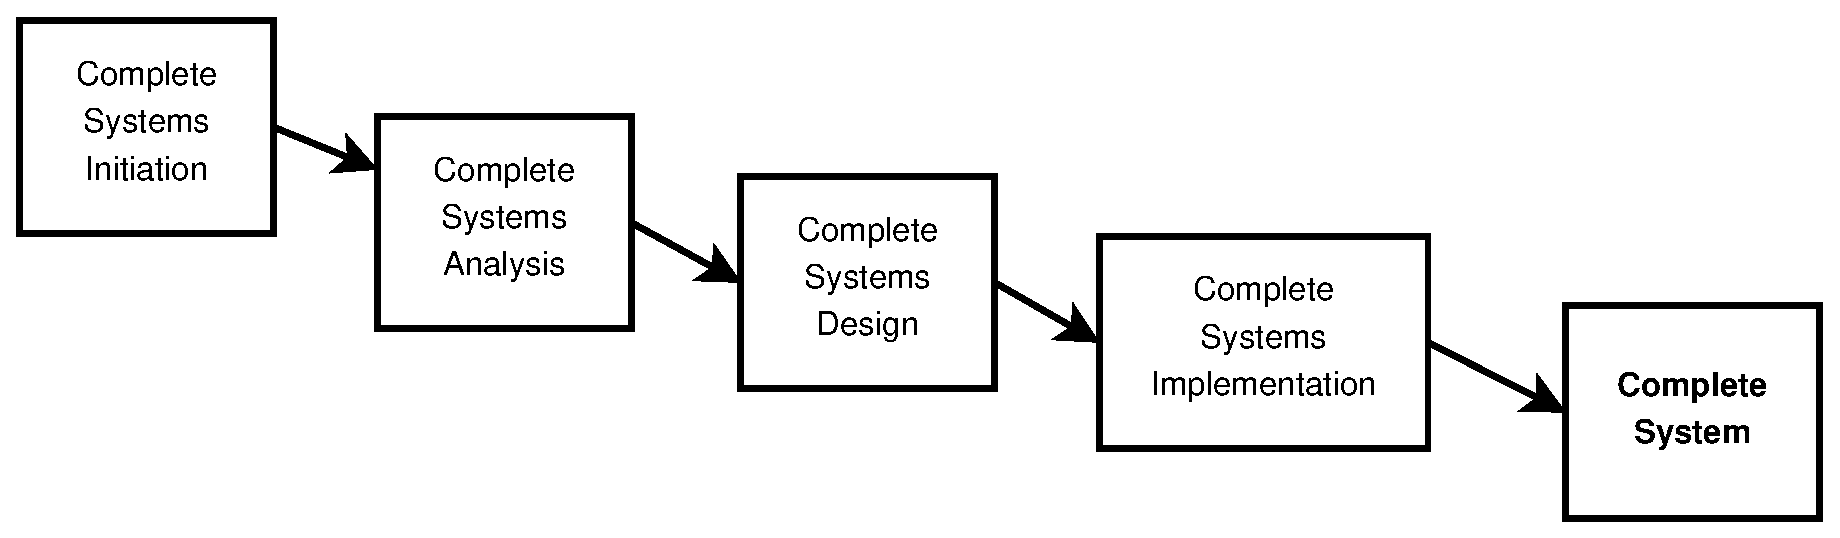
\includegraphics[width=15cm]{./Images/Sequential}
	\caption{Sequential/Waterfall Methodology}
	\label{fig:Sequential}
\end{center}
\end{figure}

Figure \ref{fig:Iterative} shows an iterative step methodology. This methodology means that the end user can see progress on software throughout the design of the software as he will be involved in the testing of each partial system produced. This allows for more constant communication between the end users and the software programmers, meaning that the end product is likely to be more throughly tested than a sequentially designed piece of software.

\begin{figure}[htp]
\begin{center}
	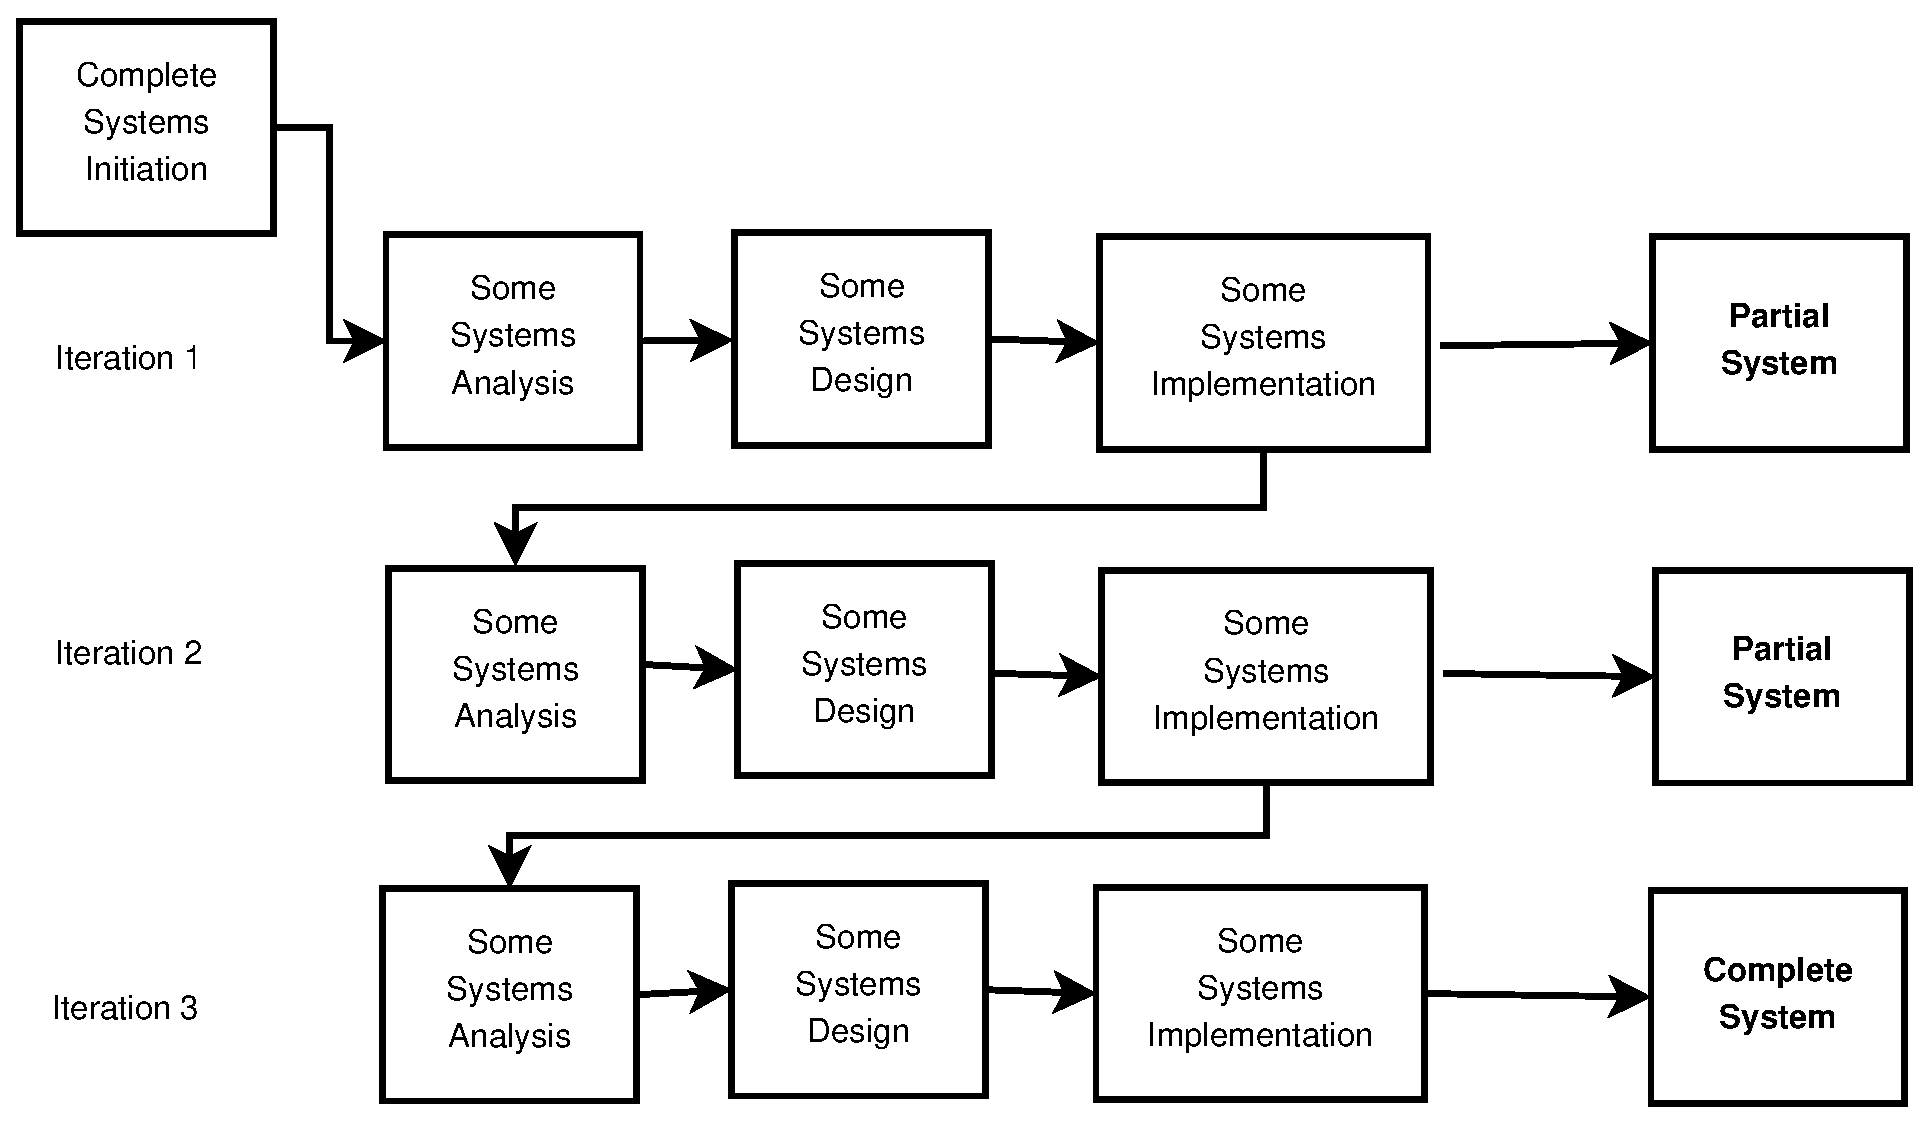
\includegraphics[width=15cm]{./Images/Iterative}
	\caption{Iterative/Incremental Methodology}
	\label{fig:Iterative}
\end{center}
\end{figure}

\subsubsection{RAD}
Rapid Application Development or RAD, is an iterative design methodology as it name implies, for the rapid development of software. It focuses on getting the end users interacting with the program during the development so that each cycle or iteration can be tested. The principle behind the beta versions and prototyping is that users will have a better idea of what they want when they see part of the program already working. RAD focuses on a few main points.
\begin{itemize}
\item Emphasis is on reducing time therefore phases of design and programming are consolidated and accelerated.
\item In each iteration, only some design specifications will be considered.
\item Assumption is that errors will be corrected in the next iteration.
\item After each iteration, end users are invited to test the software.
\item Based on feedback, designers will make changes until a version is deemed worthy of implementation.
\end{itemize}
The design phase within a RAD methodology is very short - the majority of design is done during each iteration.

\subsubsection{Agile}
In 2002, a publication by VTT Publications stated that agile software development was an umbrella term for various different software methodologies \citep{abrahamsson2002agile}. All of them share the same principles of quick iterative design, similar to the RAD methodology described above. In 2001, an manifesto was setup to document what an Agile methodology should consist of. This can be found at the Agile manifesto page \citep{Beck2001}. This states the following principles:
\begin{enumerate}
\item Individuals and interaction over process and tools
\item Working software over comprehensive documentation
\item Customer collaboration over contract negotiation
\item Responding to change over following a plan
\end{enumerate}
These principles mean the various methodologies that fall under the Agile umbrella all share common roots.
\\
\\
Of the Agile methods, there are a few which stand out as being more common than other methodologies \citep{cohen2003agile}. One of these is XP or Extreme Programming, put forward by Beck \citep{beck2000extreme} and the other is Scrum, first described in 1986 \citep{takeuchi1986new}.

\subsubsection{XP}
Extreme programming is focussed on small team developments, with 2-10 people involved in the design team. XP seeks to prevent schedule slips by having short release cycles on software \citep{beck2000extreme}. However, due to the nature of the methodology, of inter team communication and the need for co-location of the the design teams. It also has a very short iteration time of of about 2 to 4 weeks.

\subsubsection{Scrum}
Scrum is another team driven methodology that relies on an iterative, incremental steps. Scrum relies on:
\begin{itemize}
\item Transparency - Ensures that all aspects that affect the outcome are visible to those managing the work.
\item Inspection - Work must be inspected frequently.
\item Adaption - If an inspection determines something is outside acceptable limits, the inspector will adjust the process.
\end{itemize}
This list was taken from \citep{Schwaber2010}. The roles in a Scrum are those of the team (the programmers) and the ScrumMaster. The team are designed to optimise flexibility and productivity. Iterations are called sprints and these sprints are time boxed (done within a set time limit). During the sprint, the ScrumMaster makes sure that no changes are made that would affect the Sprint Goal. As the Sprints progress, the iterations come together to form the final product.

% Remove all below this line when creating thesis from Master Document
%TC:ignore
% Sets Texcount to Ignore

\addcontentsline{toc}{section}{Bibliography}
\bibliographystyle{custom}
\bibliography{../../Bibliography}

\end{document}